
% This is a simple template for a LaTeX document using the "article" class.
% See "book", "report", "letter" for other types of document.

\documentclass[10pt]{article} % use larger type; default would be 10pt

\usepackage[T1]{fontenc}
% \usepackage[french]{babel}
\usepackage[utf8]{inputenc} % set input encoding (not needed with XeLaTeX)
\usepackage{kpfonts}
\usepackage{hyperref}
\usepackage{epigraph}
\usepackage[french]{babel}
\usepackage{listings}
\usepackage{theorem}

\newtheorem{definition}{Définition}[subsection]

%%% Examples of Article customizations
% These packages are optional, depending whether you want the features they provide.
% See the LaTeX Companion or other references for full information.

%%% PAGE DIMENSIONS
\usepackage{geometry} % to change the page dimensions
\geometry{a4paper} % or letterpaper (US) or a5paper or....
% THE MARGINS FOR DSA is 1.5cm
\geometry{margin=1in}
% \geometry{margin=1.5cm} % for example, change the margins to 2 inches all round
% \geometry{landscape} % set up the page for landscape
%   read geometry.pdf for detailed page layout information


% \usepackage[parfill]{parskip} % Activate to begin paragraphs with an empty line rather than an indent

%%% PACKAGES
\usepackage{booktabs} % for much better looking tables
\usepackage{array} % for better arrays (eg matrices) in maths
\usepackage{paralist} % very flexible & customisable lists (eg. enumerate/itemize, etc.)
\usepackage{verbatim} % adds environment for commenting out blocks of text & for better verbatim
% \usepackage{subfig} % make it possible to include more than one captioned figure/table in a single float
% These packages are all incorporated in the memoir class to one degree or another...

%%% HEADERS & FOOTERS
\usepackage{fancyhdr} % This should be set AFTER setting up the page geometry
% \pagestyle{fancy} % options: empty , plain , fancy

\usepackage{graphicx} % support the \includegraphics command and options
\usepackage{subcaption}
\usepackage{caption}

\usepackage{dingbat} % For the pointy hands
\usepackage{pifont}
% \usepackage{xcolor} % For pretty colors
\usepackage[table]{xcolor}
\usepackage{tikz} % for nice pictures
\usepackage{blindtext}
\usepackage{wrapfig}
\usepackage{gensymb}
% \usepackage{table}

% COLORs
\definecolor{mygold}{RGB}{182, 153, 45}
\definecolor{mygreen}{RGB}{62, 171, 0}
\definecolor{dullgreen}{RGB}{165, 181, 45}
\definecolor{mypurp}{RGB}{84, 45, 181}


% \renewcommand{\headrule}{\color{gray}}
\renewcommand{\headrule}{\hbox to\headwidth{%
  \color{gray}\leaders\hrule height \headrulewidth\hfill}}

\renewcommand{\footrulewidth}{1pt}
% \renewcommand{\footrule}{\hbox to\headwirth{
%     \color{gray}\leaders\hrule height \footrulewidth\hfill}}

\renewcommand{\footrule}{{\color{gray}\vskip-\footruleskip\vskip-\footrulewidth \hrule width\headwidth height\footrulewidth\vskip\footruleskip}}

\fancyhf{}
% \rhead{\textcolor{gray}{Séance TP 1}}
\chead{\color{gray} Câbles Sous-marin}
% \lhead{Optimisation du GCC}
% \lfoot{\color{gray}\textcopyright 2022 Evan Voyles}
% \rfoot{\color{gray} Page \thepage\ sur 3}
\cfoot{\color{gray}Spécialité MAIN-3}
% \footskip = 0pt
% \voffset = 10pt
% \headsep = 0pt
% \cfoot{\thepage\ of \pageref{LastPage}}

% \renewcommand{\headrulewidth}{0pt} % customise the layout...
% \lhead{}\chead{}\rhead{}
% \lfoot{}\cfoot{\thepage}\rfoot{}

% \usepackage{}
\usepackage[absolute,overlay]{textpos} % Add text in any arbitrary position
% \usepackage{biblatex}

%%% SECTION TITLE APPEARANCE
\usepackage{sectsty}
\allsectionsfont{\sffamily\mdseries\upshape} % (See the fntguide.pdf for font help)
% (This matches ConTeXt defaults)

%%% ToC (table of contents) APPEARANCE
\usepackage[nottoc,notlof,notlot]{tocbibind} % Put the bibliography in the ToC
\usepackage[titles,subfigure]{tocloft} % Alter the style of the Table of Contents
\renewcommand{\cftsecfont}{\rmfamily\mdseries\upshape}
\renewcommand{\cftsecpagefont}{\rmfamily\mdseries\upshape} % No bold!

%%% END Article customizations

%%% The "real" document content comes below...

\newcommand{\asgold}[1]{\textcolor{mygold}{{\bf#1}}}
\newcommand{\asgrey}[1]{\textcolor{gray}{{\bf#1}}}
\newcommand{\asred}[1]{\textcolor{red}{{\bf#1}}}
\newcommand{\asor}[1]{\textcolor{orange}{{\bf#1}}}
\newcommand{\ascy}[1]{\textcolor{cyan}{{\bf#1}}}
\newcommand{\asgr}[1]{\textcolor{mygreen}{{\bf#1}}}
\newcommand{\aspurp}[1]{\textcolor{mypurp}{{\bf#1}}}

%%% LSTLISTINGS CONFIG:
\lstset{ %
  backgroundcolor=\color{white},   % choose the background color; you must add \usepackage{color} or \usepackage{xcolor}
  basicstyle=\footnotesize,        % the size of the fonts that are used for the code
  breakatwhitespace=false,         % sets if automatic breaks should only happen at whitespace
  breaklines=true,                 % sets automatic line breaking
  captionpos=b,                    % sets the caption-position to bottom
  commentstyle=\color{red}\textit,    % comment style
  deletekeywords={set, min, max, seq},            % if you want to delete keywords from the given language
  escapeinside={\%*}{*)},          % if you want to add LaTeX within your code
  extendedchars=true,              % lets you use non-ASCII characters; for 8-bits encodings only, does not work with UTF-8
  frame=tb,	                   	   % adds a frame around the code
  keepspaces=true,                 % keeps spaces in text, useful for keeping indentation of code (possibly needs columns=flexible)
  keywordstyle=\color{blue}\bfseries,       % keyword style
  language=R,                 % the language of the code (can be overrided per snippet)
  otherkeywords={*,...},           % if you want to add more keywords to the set
  numbers=left,                    % where to put the line-numbers; possible values are (none, left, right)
  numbersep=5pt,                   % how far the line-numbers are from the code
  numberstyle=\tiny\color{green}, % the style that is used for the line-numbers
  rulecolor=\color{black},         % if not set, the frame-color may be changed on line-breaks within not-black text (e.g. comments (green here))
  showspaces=false,                % show spaces everywhere adding particular underscores; it overrides 'showstringspaces'
  showstringspaces=false,          % underline spaces within strings only
  showtabs=false,                  % show tabs within strings adding particular underscores
  stepnumber=1,                    % the step between two line-numbers. If it's 1, each line will be numbered
  stringstyle=\color{purple}, % string literal style
  tabsize=2,	                   % sets default tabsize to 2 spaces
  title=\lstname,                  % show the filename of files included with \lstinputlisting; also try caption instead of title
  columns=fixed                    % Using fixed column width (for e.g. nice alignment)
}

\title{Simulation conditionnelle d’un processus gaussien}
\author{NEEL Pauline, PETROS Russom Samson, RAKOTOVAO Jonathan, VOYLES Evan}
\date{15 Mars 2022}


\begin{document}


\begin{titlepage}

\maketitle

\begin{figure}[h!]
    \centering
    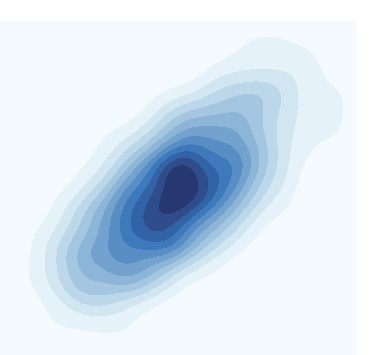
\includegraphics{media/plot.png}
\end{figure}

\vspace{3cm}

% \begin{figure}[h!]
%     \centering
%     
\includegraphics[width=0.25\linewidth]{media/1280px-Logo_Polytech_Sorbonne.png}
% \end{figure}

% \begin{abstract}
% Abstract.

% \end{abstract}

% \renewcommand {\epigraphflush} {center}

\epigraph{Any one who considers arithmetical methods of producing random digits is, of course, in a state of sin}
 {\textit{John von Neumann}}

\newpage

\end{titlepage}

\pagestyle{fancy}

\section{Génération de variables aléatoires}

Un ordinateur n'est qu'un gros agencement complexe de circuits. Regnées par les lois physiques, les opérations provenant du mouvement des électrons
sont encodées par les fonctions booléennes. Les \textit{fonctions} - dans le sens mathématique - sont des objets purement déterministes. Autrement dit,
une fonction associe à une donnée d'entrée, une unique valeur dans l'espace d'arrivée. Si on lui donne plusieurs fois la même valeur, par exemple $x_1$ et $x_2$
telles que $x_1 = x_2$, la définition d'une fonction implique que $f(x_1) = f(x_2)$. D'où vient l'énigme : Comment générer des variables aléatoires alors que nous
disposons seulement de méthodes déterministes?
% \setlength \epigraphwidth {\linewidth}

Nous ne pouvons pas à répondre à cette question plus éloquemment que le fait John von Neumann, l'un des meilleurs mathémathiciens, pionniers, informaticiens de tous les temps; générer des variables aléatoires sur un ordinateur est tout simplement impossible.
Cependant, cela ne nous empêchera pas d'essayer quand même. Il s'agira de produire des variables dites pseudo-aléatoires.

\section{Loi uniforme}

On commence notre projet en étudiant la loi la plus simple parmi les lois usuelles - la loi uniforme. Tout d'abord, parce qu'elle est simple, mais la loi uniforme va également nous permettre construire des algorithmes plus complexes, notamment la méthode de la transormée inverse ou la méthode de rejet. Ainsi, cela nous permettra de simuler différentes lois, comme la loi normale, la loi exponentielle, etc. Il s'agira principalement d'échantilloner une variable $X\sim \mathcal{U}(0, 1)$ puis ensuite d'effectuer des manipulations mathématiques pour produire une variable suivant une autre loi ciblée.

Alors sans plus tarder, on formalise nos objectifs. Le principe est le suivant: nous allons générer une suite $(x_n$) à partir d'une graine $x_0$ et une fonction $f : \mathbb{R} \longrightarrow \mathbb{R}$ telle que
$$
\left\{
    \begin{array}{ll}
        x_{0} \in \mathbb{R} \\
        x_{n} = f(x_{n - 1})  \quad \forall n \in \mathbb{N} \\
    \end{array}
\right.
$$

On souhaite trouver une fonction qui vérifie certaines qualités désirées. Par exemple, on veut que notre fonction ait une période suffisamment longue. En effet, nous savons qu'elle sera périodique, il est donc importante que se période soit très grande pour pas qu'un schéma soit visible. On souhiate également qu'elle
produise des valeurs uniformément réparties sur un intervalle. Etudions la fonction $x \mapsto (x + 1) \mathbin{\%} 2$, où \% est l'opération de modulos et on fixe une graine $x_0 = 1$.
\begin{align*}
    f(x_0) &= (1 + 1) \mathbin{\%} 2 = 2 \mathbin{\%} 2 = 0 \\
    f(x_1) &= (0 + 1) \mathbin{\%} 2 = 1 \mathbin{\%} 2 = 1 \\
    f(x_2) &= (1 + 1) = 0
\end{align*}
Cette fonction produit alors la suite
\begin{equation*}
    \{1, 0, 1, 0, 1, 0, 1, 0, ...\}
\end{equation*}
dont la période est 2 et évidemment dont les valeurs ne sont pas aussi variées qu'on le souhaite. Nous verrons plus précisement ce que
``suffisamment variés'' veut dire. Pour l'instant, on se contente de dire que cette suite-là n'atteint pas nos attentes. Heureusement pour nous, il existe de nombreuses fonctions
qui remplissent nos critères recherchés, ce sont des fonctions pseudo-aléatoires, elles sont déterminées mais leurs comportements s'approchent de l'aléatoire.

\subsection{Générateur congruentiel linéaire}

La méthode la plus directe à implémenter pour générer une telle suite est un \textit{générateur congruentiel linéaire}. Congruentiel parce qu'il s'agit d'une opération modulo et
linéaire vu qu'il y a une transformation affine. Dans le cas général, on considère les fonctions de la forme:
$$
    f(x; a, c, m) = (ax + c) \bmod m.
$$

D'ailleurs, la fonction étudiée dans la section précédente est un générateur congruentiel linéaire dont les paramètres sont $a = 1$, $c = 1$, et $m = 2$. Ne vous inquiétez pas, il existe un large panel de
générateurs congruentiels linéaires (LCG). Les choix des paramètres utilisés par les logiciels connus sont détaillés sur une page Wikipédia et leurs propriétés sont déjà
bien étudiées. Vu que l'objectif de notre projet est d'approfondir la connaissance autour des méthodes pour générer des variables (pseudo) aléatoires, on a décidé d'implémenter notre propre LCG hybride.
Pour $m$, on choisit $2^{31} - 1$, un prime mersenne qui est très connu. Pour $a$, on s'amuse en choissisant $12345678$. Finalement, on affecte à l'incrémenteur $c$ la valeur 1.
$$
    f_{sousmarin}(x) = (12345678x + 1) \bmod (2^{31} - 1)
$$


\subsection{Implémentation en R}
Dans ce projet, nous faisons le choix d'implémenter notre propre version de runif afin de comprendre en profondeur la notion d'aléatoire. En effet, toutes les autres lois que nous allons pouvoir simuler, seront constuites à partir de runif. Il était donc important pour nous de faire cette étape. Afin d'implémenter une version de notre fonction en language de programmation R, on doit s'éloigner un peu de la pureté de la théorie et se salir les mains dans le code ! C'est-à-dire que l'on ne va pas garder une valeur $x_0$
pour toute l'éternité; on aura une variable globale déterminant l'état du générateur qui serait mise à jour quand on veut générer une suite de valeurs.

% \lstset{language=R, caption=somecaption, keywords={smooth}}

\begin{lstlisting}[language =R]

    # Initialiser la graine (une variable globale) a 0
    g_SEED_SOUSMARIN <- 0

    # similaire a la fonction de R set.seed, mettre a jour
    # la valeur de g_SEED_SOUSMARIN
    set_seed <- function(seed) {
        assign("g_SEED_SOUSMARIN", seed, envir = .GlobalEnv)
    }

    # La fonction LCG pure qu'on a definie en partie 3
    f_sousmarin <- function(x) {
        (12345678 * x + 1) %% (2^31 - 1)
    }

    # Generer une suite des variables de taille n en mettant a jour l'etat
    # de la graine a chaque pas.
    gen_suite <- function(n) {

        suite <- vector("numeric", n) # allouer un vecteur de taille n

        for (i in seq_len(n)) {
            x_i <- f_sousmarin(g_SEED_SOUSMARIN)
            suite[[i]] <- x_i
            set_seed(x_i)
        }

        suite
    }
\end{lstlisting}

On a donc implémenté notre propre LCG, \texttt{f\_sousmarin}. Pour renvoyer une valeur dans l'intervalle ]0, 1[ afin de simuler $X \sim \mathcal{U}(0, 1)$, on remarque que
la division modulo $m$ renvoie une valeur entre ]0, $m - 1$[. Pour le normaliser, on divise par le facteur $m - 1 \equiv 2^{31} - 2$.

\begin{lstlisting}[language=R]

    r_std_unif <- function(n) {

        suite <- vector("numeric", n)

        for (i in seq_len(n)) {
            x_i <- f_sousmarin(g_SEED_SOUSMARIN)
            suite[[i]] <- x_i / (2^31 - 2)
            set_seed(x_i)
        }

        suite
    }

\end{lstlisting}

Si on considère le cas général où l'on souhaiterait générer des variables uniformément réparties dans l'intervalle ]$a$, $b$[, on commence tout d'abord
par échantillonner $X \sim \mathcal{U}(0, 1)$. Ensuite, on multiplie $X$ par l'écart entre $a$ et $b$, ($b - a$), pour produire une variable $X_{b - a} \in$ ]$0$, $b - a$[. Finalement,
on décale $X_{b - a}$ en additionnant $a$ pour finir avec la variable aléatoire uniformément répartie dans l'intervalle ]$0 + a, b - a + a$[ $\equiv $ ]$a, b$[. Après cette transformation affine appliquée à
$X$, nous avons $X_{a,b} \sim \mathcal{U}(a, b)$.

On imite le comportement et la signature de la fonction dans R de base \texttt{runif} avec l'implémentation suivante

\begin{lstlisting}[language=R]

    r_unif <- function(n, min = 0, max = 1) {

        spread <- max - min
        suite  <- vector("numeric", n)

        for (i in seq_len(n)) {
            x_i <- f_sousmarin(g_SEED_SOUSMARIN)
            suite[[i]] <- (x_i * spread) / (2^31 - 2) + min
            set_seed(x_i)
        }

        suite
    }

\end{lstlisting}


\subsection{Vérification pour la loi uniforme}

Comment vérifier que notre LCG produit des valeurs qui sont véritablement réparties uniformément ? Quand il s'agit de produire
des milliards d'observations, on ne peut pas facilement vérifier à la main si notre fonction n'a pas de structure évidente (sauf la période qui est mathématiquement inévitable).
Pourtant, on peut commencer avec une exploration visuelle.

Pour ce faire, on utilise la fonction \texttt{r\_std\_unif} définie au-dessus pour générer 1E6 valeurs aléatoires qui sont supposées être uniformément
réparties sur l'intervalle ]$0, 1$[.

\begin{figure}[h!]
    \centering
    % Created by tikzDevice version 0.12.3.1 on 2022-03-15 02:59:11
% !TEX encoding = UTF-8 Unicode
\begin{tikzpicture}[x=1pt,y=1pt]
\definecolor{fillColor}{RGB}{255,255,255}
\path[use as bounding box,fill=fillColor,fill opacity=0.00] (0,0) rectangle (361.35,216.81);
\begin{scope}
\path[clip] (  0.00,  0.00) rectangle (361.35,216.81);
\definecolor{drawColor}{RGB}{255,255,255}
\definecolor{fillColor}{RGB}{255,255,255}

\path[draw=drawColor,line width= 0.6pt,line join=round,line cap=round,fill=fillColor] (  0.00,  0.00) rectangle (361.35,216.81);
\end{scope}
\begin{scope}
\path[clip] ( 44.91, 30.69) rectangle (355.85,211.31);
\definecolor{fillColor}{gray}{0.92}

\path[fill=fillColor] ( 44.91, 30.69) rectangle (355.85,211.31);
\definecolor{drawColor}{RGB}{255,255,255}

\path[draw=drawColor,line width= 0.3pt,line join=round] ( 44.91, 71.16) --
	(355.85, 71.16);

\path[draw=drawColor,line width= 0.3pt,line join=round] ( 44.91,135.70) --
	(355.85,135.70);

\path[draw=drawColor,line width= 0.3pt,line join=round] ( 44.91,200.23) --
	(355.85,200.23);

\path[draw=drawColor,line width= 0.3pt,line join=round] ( 94.38, 30.69) --
	( 94.38,211.31);

\path[draw=drawColor,line width= 0.3pt,line join=round] (165.05, 30.69) --
	(165.05,211.31);

\path[draw=drawColor,line width= 0.3pt,line join=round] (235.71, 30.69) --
	(235.71,211.31);

\path[draw=drawColor,line width= 0.3pt,line join=round] (306.38, 30.69) --
	(306.38,211.31);

\path[draw=drawColor,line width= 0.6pt,line join=round] ( 44.91, 38.90) --
	(355.85, 38.90);

\path[draw=drawColor,line width= 0.6pt,line join=round] ( 44.91,103.43) --
	(355.85,103.43);

\path[draw=drawColor,line width= 0.6pt,line join=round] ( 44.91,167.97) --
	(355.85,167.97);

\path[draw=drawColor,line width= 0.6pt,line join=round] ( 59.04, 30.69) --
	( 59.04,211.31);

\path[draw=drawColor,line width= 0.6pt,line join=round] (129.71, 30.69) --
	(129.71,211.31);

\path[draw=drawColor,line width= 0.6pt,line join=round] (200.38, 30.69) --
	(200.38,211.31);

\path[draw=drawColor,line width= 0.6pt,line join=round] (271.05, 30.69) --
	(271.05,211.31);

\path[draw=drawColor,line width= 0.6pt,line join=round] (341.72, 30.69) --
	(341.72,211.31);
\definecolor{drawColor}{RGB}{0,0,0}
\definecolor{fillColor}{RGB}{16,118,212}

\path[draw=drawColor,line width= 0.6pt,line cap=rect,fill=fillColor] ( 59.04, 38.90) rectangle ( 62.58,201.64);

\path[draw=drawColor,line width= 0.6pt,line cap=rect,fill=fillColor] ( 62.58, 38.90) rectangle ( 66.11,199.58);

\path[draw=drawColor,line width= 0.6pt,line cap=rect,fill=fillColor] ( 66.11, 38.90) rectangle ( 69.64,200.31);

\path[draw=drawColor,line width= 0.6pt,line cap=rect,fill=fillColor] ( 69.64, 38.90) rectangle ( 73.18,200.42);

\path[draw=drawColor,line width= 0.6pt,line cap=rect,fill=fillColor] ( 73.18, 38.90) rectangle ( 76.71,200.22);

\path[draw=drawColor,line width= 0.6pt,line cap=rect,fill=fillColor] ( 76.71, 38.90) rectangle ( 80.24,202.65);

\path[draw=drawColor,line width= 0.6pt,line cap=rect,fill=fillColor] ( 80.24, 38.90) rectangle ( 83.78,196.18);

\path[draw=drawColor,line width= 0.6pt,line cap=rect,fill=fillColor] ( 83.78, 38.90) rectangle ( 87.31,201.56);

\path[draw=drawColor,line width= 0.6pt,line cap=rect,fill=fillColor] ( 87.31, 38.90) rectangle ( 90.84,198.76);

\path[draw=drawColor,line width= 0.6pt,line cap=rect,fill=fillColor] ( 90.84, 38.90) rectangle ( 94.38,197.69);

\path[draw=drawColor,line width= 0.6pt,line cap=rect,fill=fillColor] ( 94.38, 38.90) rectangle ( 97.91,200.16);

\path[draw=drawColor,line width= 0.6pt,line cap=rect,fill=fillColor] ( 97.91, 38.90) rectangle (101.44,199.52);

\path[draw=drawColor,line width= 0.6pt,line cap=rect,fill=fillColor] (101.44, 38.90) rectangle (104.98,202.58);

\path[draw=drawColor,line width= 0.6pt,line cap=rect,fill=fillColor] (104.98, 38.90) rectangle (108.51,199.11);

\path[draw=drawColor,line width= 0.6pt,line cap=rect,fill=fillColor] (108.51, 38.90) rectangle (112.04,200.25);

\path[draw=drawColor,line width= 0.6pt,line cap=rect,fill=fillColor] (112.04, 38.90) rectangle (115.58,201.56);

\path[draw=drawColor,line width= 0.6pt,line cap=rect,fill=fillColor] (115.58, 38.90) rectangle (119.11,200.07);

\path[draw=drawColor,line width= 0.6pt,line cap=rect,fill=fillColor] (119.11, 38.90) rectangle (122.64,200.07);

\path[draw=drawColor,line width= 0.6pt,line cap=rect,fill=fillColor] (122.64, 38.90) rectangle (126.18,198.81);

\path[draw=drawColor,line width= 0.6pt,line cap=rect,fill=fillColor] (126.18, 38.90) rectangle (129.71,202.02);

\path[draw=drawColor,line width= 0.6pt,line cap=rect,fill=fillColor] (129.71, 38.90) rectangle (133.24,197.73);

\path[draw=drawColor,line width= 0.6pt,line cap=rect,fill=fillColor] (133.24, 38.90) rectangle (136.78,201.95);

\path[draw=drawColor,line width= 0.6pt,line cap=rect,fill=fillColor] (136.78, 38.90) rectangle (140.31,199.94);

\path[draw=drawColor,line width= 0.6pt,line cap=rect,fill=fillColor] (140.31, 38.90) rectangle (143.84,197.50);

\path[draw=drawColor,line width= 0.6pt,line cap=rect,fill=fillColor] (143.84, 38.90) rectangle (147.38,200.54);

\path[draw=drawColor,line width= 0.6pt,line cap=rect,fill=fillColor] (147.38, 38.90) rectangle (150.91,201.90);

\path[draw=drawColor,line width= 0.6pt,line cap=rect,fill=fillColor] (150.91, 38.90) rectangle (154.45,200.02);

\path[draw=drawColor,line width= 0.6pt,line cap=rect,fill=fillColor] (154.45, 38.90) rectangle (157.98,200.72);

\path[draw=drawColor,line width= 0.6pt,line cap=rect,fill=fillColor] (157.98, 38.90) rectangle (161.51,199.56);

\path[draw=drawColor,line width= 0.6pt,line cap=rect,fill=fillColor] (161.51, 38.90) rectangle (165.05,201.76);

\path[draw=drawColor,line width= 0.6pt,line cap=rect,fill=fillColor] (165.05, 38.90) rectangle (168.58,199.36);

\path[draw=drawColor,line width= 0.6pt,line cap=rect,fill=fillColor] (168.58, 38.90) rectangle (172.11,201.63);

\path[draw=drawColor,line width= 0.6pt,line cap=rect,fill=fillColor] (172.11, 38.90) rectangle (175.65,203.10);

\path[draw=drawColor,line width= 0.6pt,line cap=rect,fill=fillColor] (175.65, 38.90) rectangle (179.18,199.76);

\path[draw=drawColor,line width= 0.6pt,line cap=rect,fill=fillColor] (179.18, 38.90) rectangle (182.71,200.47);

\path[draw=drawColor,line width= 0.6pt,line cap=rect,fill=fillColor] (182.71, 38.90) rectangle (186.25,200.09);

\path[draw=drawColor,line width= 0.6pt,line cap=rect,fill=fillColor] (186.25, 38.90) rectangle (189.78,197.78);

\path[draw=drawColor,line width= 0.6pt,line cap=rect,fill=fillColor] (189.78, 38.90) rectangle (193.31,198.20);

\path[draw=drawColor,line width= 0.6pt,line cap=rect,fill=fillColor] (193.31, 38.90) rectangle (196.85,200.72);

\path[draw=drawColor,line width= 0.6pt,line cap=rect,fill=fillColor] (196.85, 38.90) rectangle (200.38,196.53);

\path[draw=drawColor,line width= 0.6pt,line cap=rect,fill=fillColor] (200.38, 38.90) rectangle (203.91,199.83);

\path[draw=drawColor,line width= 0.6pt,line cap=rect,fill=fillColor] (203.91, 38.90) rectangle (207.45,196.34);

\path[draw=drawColor,line width= 0.6pt,line cap=rect,fill=fillColor] (207.45, 38.90) rectangle (210.98,198.52);

\path[draw=drawColor,line width= 0.6pt,line cap=rect,fill=fillColor] (210.98, 38.90) rectangle (214.51,202.13);

\path[draw=drawColor,line width= 0.6pt,line cap=rect,fill=fillColor] (214.51, 38.90) rectangle (218.05,199.05);

\path[draw=drawColor,line width= 0.6pt,line cap=rect,fill=fillColor] (218.05, 38.90) rectangle (221.58,198.47);

\path[draw=drawColor,line width= 0.6pt,line cap=rect,fill=fillColor] (221.58, 38.90) rectangle (225.11,201.41);

\path[draw=drawColor,line width= 0.6pt,line cap=rect,fill=fillColor] (225.11, 38.90) rectangle (228.65,200.03);

\path[draw=drawColor,line width= 0.6pt,line cap=rect,fill=fillColor] (228.65, 38.90) rectangle (232.18,197.60);

\path[draw=drawColor,line width= 0.6pt,line cap=rect,fill=fillColor] (232.18, 38.90) rectangle (235.71,198.92);

\path[draw=drawColor,line width= 0.6pt,line cap=rect,fill=fillColor] (235.71, 38.90) rectangle (239.25,201.38);

\path[draw=drawColor,line width= 0.6pt,line cap=rect,fill=fillColor] (239.25, 38.90) rectangle (242.78,202.66);

\path[draw=drawColor,line width= 0.6pt,line cap=rect,fill=fillColor] (242.78, 38.90) rectangle (246.31,201.89);

\path[draw=drawColor,line width= 0.6pt,line cap=rect,fill=fillColor] (246.31, 38.90) rectangle (249.85,201.23);

\path[draw=drawColor,line width= 0.6pt,line cap=rect,fill=fillColor] (249.85, 38.90) rectangle (253.38,201.76);

\path[draw=drawColor,line width= 0.6pt,line cap=rect,fill=fillColor] (253.38, 38.90) rectangle (256.91,200.63);

\path[draw=drawColor,line width= 0.6pt,line cap=rect,fill=fillColor] (256.91, 38.90) rectangle (260.45,201.53);

\path[draw=drawColor,line width= 0.6pt,line cap=rect,fill=fillColor] (260.45, 38.90) rectangle (263.98,198.80);

\path[draw=drawColor,line width= 0.6pt,line cap=rect,fill=fillColor] (263.98, 38.90) rectangle (267.51,200.78);

\path[draw=drawColor,line width= 0.6pt,line cap=rect,fill=fillColor] (267.51, 38.90) rectangle (271.05,199.24);

\path[draw=drawColor,line width= 0.6pt,line cap=rect,fill=fillColor] (271.05, 38.90) rectangle (274.58,202.75);

\path[draw=drawColor,line width= 0.6pt,line cap=rect,fill=fillColor] (274.58, 38.90) rectangle (278.11,199.77);

\path[draw=drawColor,line width= 0.6pt,line cap=rect,fill=fillColor] (278.11, 38.90) rectangle (281.65,200.09);

\path[draw=drawColor,line width= 0.6pt,line cap=rect,fill=fillColor] (281.65, 38.90) rectangle (285.18,202.83);

\path[draw=drawColor,line width= 0.6pt,line cap=rect,fill=fillColor] (285.18, 38.90) rectangle (288.72,200.27);

\path[draw=drawColor,line width= 0.6pt,line cap=rect,fill=fillColor] (288.72, 38.90) rectangle (292.25,198.52);

\path[draw=drawColor,line width= 0.6pt,line cap=rect,fill=fillColor] (292.25, 38.90) rectangle (295.78,201.05);

\path[draw=drawColor,line width= 0.6pt,line cap=rect,fill=fillColor] (295.78, 38.90) rectangle (299.32,200.53);

\path[draw=drawColor,line width= 0.6pt,line cap=rect,fill=fillColor] (299.32, 38.90) rectangle (302.85,202.20);

\path[draw=drawColor,line width= 0.6pt,line cap=rect,fill=fillColor] (302.85, 38.90) rectangle (306.38,199.52);

\path[draw=drawColor,line width= 0.6pt,line cap=rect,fill=fillColor] (306.38, 38.90) rectangle (309.92,199.32);

\path[draw=drawColor,line width= 0.6pt,line cap=rect,fill=fillColor] (309.92, 38.90) rectangle (313.45,200.34);

\path[draw=drawColor,line width= 0.6pt,line cap=rect,fill=fillColor] (313.45, 38.90) rectangle (316.98,202.40);

\path[draw=drawColor,line width= 0.6pt,line cap=rect,fill=fillColor] (316.98, 38.90) rectangle (320.52,199.86);

\path[draw=drawColor,line width= 0.6pt,line cap=rect,fill=fillColor] (320.52, 38.90) rectangle (324.05,202.24);

\path[draw=drawColor,line width= 0.6pt,line cap=rect,fill=fillColor] (324.05, 38.90) rectangle (327.58,200.63);

\path[draw=drawColor,line width= 0.6pt,line cap=rect,fill=fillColor] (327.58, 38.90) rectangle (331.12,199.31);

\path[draw=drawColor,line width= 0.6pt,line cap=rect,fill=fillColor] (331.12, 38.90) rectangle (334.65,200.42);

\path[draw=drawColor,line width= 0.6pt,line cap=rect,fill=fillColor] (334.65, 38.90) rectangle (338.18,200.92);

\path[draw=drawColor,line width= 0.6pt,line cap=rect,fill=fillColor] (338.18, 38.90) rectangle (341.72,201.19);
\end{scope}
\begin{scope}
\path[clip] (  0.00,  0.00) rectangle (361.35,216.81);
\definecolor{drawColor}{gray}{0.30}

\node[text=drawColor,anchor=base east,inner sep=0pt, outer sep=0pt, scale=  0.88] at ( 39.96, 35.87) {0};

\node[text=drawColor,anchor=base east,inner sep=0pt, outer sep=0pt, scale=  0.88] at ( 39.96,100.40) {5000};

\node[text=drawColor,anchor=base east,inner sep=0pt, outer sep=0pt, scale=  0.88] at ( 39.96,164.94) {10000};
\end{scope}
\begin{scope}
\path[clip] (  0.00,  0.00) rectangle (361.35,216.81);
\definecolor{drawColor}{gray}{0.20}

\path[draw=drawColor,line width= 0.6pt,line join=round] ( 42.16, 38.90) --
	( 44.91, 38.90);

\path[draw=drawColor,line width= 0.6pt,line join=round] ( 42.16,103.43) --
	( 44.91,103.43);

\path[draw=drawColor,line width= 0.6pt,line join=round] ( 42.16,167.97) --
	( 44.91,167.97);
\end{scope}
\begin{scope}
\path[clip] (  0.00,  0.00) rectangle (361.35,216.81);
\definecolor{drawColor}{gray}{0.20}

\path[draw=drawColor,line width= 0.6pt,line join=round] ( 59.04, 27.94) --
	( 59.04, 30.69);

\path[draw=drawColor,line width= 0.6pt,line join=round] (129.71, 27.94) --
	(129.71, 30.69);

\path[draw=drawColor,line width= 0.6pt,line join=round] (200.38, 27.94) --
	(200.38, 30.69);

\path[draw=drawColor,line width= 0.6pt,line join=round] (271.05, 27.94) --
	(271.05, 30.69);

\path[draw=drawColor,line width= 0.6pt,line join=round] (341.72, 27.94) --
	(341.72, 30.69);
\end{scope}
\begin{scope}
\path[clip] (  0.00,  0.00) rectangle (361.35,216.81);
\definecolor{drawColor}{gray}{0.30}

\node[text=drawColor,anchor=base,inner sep=0pt, outer sep=0pt, scale=  0.88] at ( 59.04, 19.68) {0.00};

\node[text=drawColor,anchor=base,inner sep=0pt, outer sep=0pt, scale=  0.88] at (129.71, 19.68) {0.25};

\node[text=drawColor,anchor=base,inner sep=0pt, outer sep=0pt, scale=  0.88] at (200.38, 19.68) {0.50};

\node[text=drawColor,anchor=base,inner sep=0pt, outer sep=0pt, scale=  0.88] at (271.05, 19.68) {0.75};

\node[text=drawColor,anchor=base,inner sep=0pt, outer sep=0pt, scale=  0.88] at (341.72, 19.68) {1.00};
\end{scope}
\begin{scope}
\path[clip] (  0.00,  0.00) rectangle (361.35,216.81);
\definecolor{drawColor}{RGB}{0,0,0}

\node[text=drawColor,anchor=base,inner sep=0pt, outer sep=0pt, scale=  1.10] at (200.38,  7.64) {x};
\end{scope}
\begin{scope}
\path[clip] (  0.00,  0.00) rectangle (361.35,216.81);
\definecolor{drawColor}{RGB}{0,0,0}

\node[text=drawColor,rotate= 90.00,anchor=base,inner sep=0pt, outer sep=0pt, scale=  1.10] at ( 13.08,121.00) {count};
\end{scope}
\end{tikzpicture}


    \vspace{-1cm}
    \caption{Histogramme généré à partir d'un appel à \texttt{r\_std\_unif} avec $n = 1000000$. On initialise la graine de notre
    générateur avec un appel à \texttt{set\_seed(0)}.}

\end{figure}

On peut aussi facilement vérifier que les statistiques de notre échantillon correspondent bien à celles que l'on attend.

\begin{lstlisting}[language=R]
    library(sousmarin)

    set_seed(0)
    x <- r_std_unif(1E6)

    mu  <- mean(x) # 0.5000658
    sig <- std(x)  # 0.2877586
\end{lstlisting}

On réitère le simple fait qu'il n'y a \textbf{rien d'aléatoire} avec la génération de ces valeurs et que vous pouvez vérifier leur quantité en
téléchargant notre package \textbf{ICI}\footnote{On mettra ici un lien du github (voire un lien de CRAN????) et des instructions pour télécharger notre package}.

On passe à l'analyse. Avec notre échantillon $x$ de taille 1E6, le moyen de l'échantillon $\bar x = 0.50006584$ et l'écart type de l'échantillon est $s = 0.2877586$.
Comme la moyenne d'une loi uniforme est $\frac{b - a}{2} = \frac{1 - 0}{2} = 0.5$, nous sommes ravis de voir que $\bar x = 0.50006584 \sim 0.5$. Parallèlement, l'écart type
d'une loi uniforme est $\frac{b - a}{\sqrt{12}} = \frac{1 - 0}{\sqrt{12}} = 0.2886751$, ce qui est proche de notre $s = 0.2877586$.

\subsection{Diehard}

My boy George Marsaglia

\subsection{Vitesse}

Les boucles en R sont \textbf{LENTES}. Genre horriblement lentes. Pour la suite, on va implémenter les fonctions en C en utilisant le package Rcpp. Pour suivre, nous tentons d'explorer d'autres optimisations au niveau de la parallélisation. Ces améliorations nous donneront d'autres problèmes à résoudre tels que les conditions de courses - quand deux "threads" essaient d'accéder et
de modifier l'état du générateur en même temps.

\section{Projections}

Méthode de transormation inversée, méthode de rejet, Transforme Box-Muller.

\section{Methode de transformation inversee}

La methode de transformation inversee consiste a echantilloner une variable aleatoire $X \sim \mathcal{U}(0, 1)$ et utiliser l'expression analytique
de la fonction de repartition d'une loi cible. Comme la fonction de repartition $F(x$) est une fonction croissante definie sur $\mathbb{R}^n$ a des valeurs dans
$[0, 1]$, si on peut trouver une expression fermee de son inverse $F^{-1} : [0, 1] \longrightarrow \mathbb{R}$, on applique la methode de transformation inversee
afin de realiser des simulations.

Pour eclairer la methode, on va etudier la fonction de repartion de la loi exponentielle. Pour rappel, une variable aleatoire suivant une loi exponentielle de parametre
$\lambda$ a pour fonction de densite $f(x) = \lambda e^{-\lambda x}$ pour $x \geq 0$, $0$ sinon. On a fait expres de choisir cette loi parce qu'elle est muni avec une fonction de repartition aisement calculable
et, plus importamment, dont l'inverse a une expression analytique. On continue pour calculer sa fonction de repartition:
\begin{align*}
    F(x) &= \int_{-\infty}^xf(t)dt \\
    & = \int_{-\infty}^0 0 dt + \int_0^x \lambda e^{-\lambda t} dt \\
    &= 0 + \left[-e^{-\lambda t}\right]_0^x \\
    &= 1 - e^{-\lambda x}
\end{align*}

Avec cette expression on procede pour trouver l'inverse, $F^{-1}$ :
\begin{align*}
    y &= 1 - e^{-\lambda (F^{-1}(y))} \\
    e^{\lambda (F^{-1}(y))} &= 1 - y \\
    -\lambda F^{-1}(y) &= \ln(1 - y) \\
    F^{-1}(y) &= \frac{-\ln(1 - y)}{\lambda}
\end{align*}

La loi exponentielle est l'une des peu loi ou on peut facilement trouver une expression ferme de l'inverse de sa fonction de repartion. Cela nous permet
d'echantilloner une variable aleatoire $X \sim \exp(\lambda)$ efficacement a partir d'une seule realisation d'une loi uniformer. Il s'agit tout
simplement de tirer $U \sim \mathcal{U}(0, 1)$ et ensuite evaluer $X = F^{-1}(U)$.

L'implementation en R n'est qu'une seule ligne:

\begin{lstlisting}[language=R]
    rexp_inv <- function(n, lambda = 1) {
        # Generate n realizations of a uniform random variable n times
        (-1 / lambda) * log(runif(n, 0, 1))
    }
\end{lstlisting}


\section{Methode d'acceptation-rejet}

\begin{figure}[h!]
\centering
% Created by tikzDevice version 0.12.3.1 on 2022-05-10 12:46:44
% !TEX encoding = UTF-8 Unicode
\begin{tikzpicture}[x=1pt,y=1pt]
\definecolor{fillColor}{RGB}{255,255,255}
\path[use as bounding box,fill=fillColor,fill opacity=0.00] (0,0) rectangle (361.35,216.81);
\begin{scope}
\path[clip] (  0.00,  0.00) rectangle (361.35,216.81);
\definecolor{drawColor}{RGB}{255,255,255}
\definecolor{fillColor}{RGB}{255,255,255}

\path[draw=drawColor,line width= 0.6pt,line join=round,line cap=round,fill=fillColor] (  0.00,  0.00) rectangle (361.35,216.81);
\end{scope}
\begin{scope}
\path[clip] ( 36.11, 30.69) rectangle (355.85,178.94);
\definecolor{fillColor}{gray}{0.92}

\path[fill=fillColor] ( 36.11, 30.69) rectangle (355.85,178.94);
\definecolor{drawColor}{RGB}{255,255,255}

\path[draw=drawColor,line width= 0.3pt,line join=round] ( 36.11, 60.78) --
	(355.85, 60.78);

\path[draw=drawColor,line width= 0.3pt,line join=round] ( 36.11,107.99) --
	(355.85,107.99);

\path[draw=drawColor,line width= 0.3pt,line join=round] ( 36.11,155.20) --
	(355.85,155.20);

\path[draw=drawColor,line width= 0.3pt,line join=round] ( 84.41, 30.69) --
	( 84.41,178.94);

\path[draw=drawColor,line width= 0.3pt,line join=round] (157.81, 30.69) --
	(157.81,178.94);

\path[draw=drawColor,line width= 0.3pt,line join=round] (231.21, 30.69) --
	(231.21,178.94);

\path[draw=drawColor,line width= 0.3pt,line join=round] (304.62, 30.69) --
	(304.62,178.94);

\path[draw=drawColor,line width= 0.6pt,line join=round] ( 36.11, 37.17) --
	(355.85, 37.17);

\path[draw=drawColor,line width= 0.6pt,line join=round] ( 36.11, 84.38) --
	(355.85, 84.38);

\path[draw=drawColor,line width= 0.6pt,line join=round] ( 36.11,131.60) --
	(355.85,131.60);

\path[draw=drawColor,line width= 0.6pt,line join=round] ( 36.11,178.81) --
	(355.85,178.81);

\path[draw=drawColor,line width= 0.6pt,line join=round] ( 47.71, 30.69) --
	( 47.71,178.94);

\path[draw=drawColor,line width= 0.6pt,line join=round] (121.11, 30.69) --
	(121.11,178.94);

\path[draw=drawColor,line width= 0.6pt,line join=round] (194.51, 30.69) --
	(194.51,178.94);

\path[draw=drawColor,line width= 0.6pt,line join=round] (267.91, 30.69) --
	(267.91,178.94);

\path[draw=drawColor,line width= 0.6pt,line join=round] (341.32, 30.69) --
	(341.32,178.94);
\definecolor{drawColor}{RGB}{0,0,0}
\definecolor{fillColor}{RGB}{0,0,0}

\path[draw=drawColor,line width= 0.4pt,line join=round,line cap=round,fill=fillColor] ( 50.64, 38.12) circle (  0.62);

\path[draw=drawColor,line width= 0.4pt,line join=round,line cap=round,fill=fillColor] ( 53.58, 39.06) circle (  0.62);

\path[draw=drawColor,line width= 0.4pt,line join=round,line cap=round,fill=fillColor] ( 56.52, 40.95) circle (  0.62);

\path[draw=drawColor,line width= 0.4pt,line join=round,line cap=round,fill=fillColor] ( 59.45, 41.89) circle (  0.62);

\path[draw=drawColor,line width= 0.4pt,line join=round,line cap=round,fill=fillColor] ( 62.39, 44.72) circle (  0.62);

\path[draw=drawColor,line width= 0.4pt,line join=round,line cap=round,fill=fillColor] ( 65.33, 43.78) circle (  0.62);

\path[draw=drawColor,line width= 0.4pt,line join=round,line cap=round,fill=fillColor] ( 68.26, 49.45) circle (  0.62);

\path[draw=drawColor,line width= 0.4pt,line join=round,line cap=round,fill=fillColor] ( 71.20, 49.45) circle (  0.62);

\path[draw=drawColor,line width= 0.4pt,line join=round,line cap=round,fill=fillColor] ( 74.13, 46.61) circle (  0.62);

\path[draw=drawColor,line width= 0.4pt,line join=round,line cap=round,fill=fillColor] ( 77.07, 46.61) circle (  0.62);

\path[draw=drawColor,line width= 0.4pt,line join=round,line cap=round,fill=fillColor] ( 80.01, 50.39) circle (  0.62);

\path[draw=drawColor,line width= 0.4pt,line join=round,line cap=round,fill=fillColor] ( 82.94, 51.33) circle (  0.62);

\path[draw=drawColor,line width= 0.4pt,line join=round,line cap=round,fill=fillColor] ( 85.88, 53.22) circle (  0.62);

\path[draw=drawColor,line width= 0.4pt,line join=round,line cap=round,fill=fillColor] ( 88.81, 53.22) circle (  0.62);

\path[draw=drawColor,line width= 0.4pt,line join=round,line cap=round,fill=fillColor] ( 91.75, 54.17) circle (  0.62);

\path[draw=drawColor,line width= 0.4pt,line join=round,line cap=round,fill=fillColor] ( 94.69, 52.28) circle (  0.62);

\path[draw=drawColor,line width= 0.4pt,line join=round,line cap=round,fill=fillColor] ( 97.62, 62.67) circle (  0.62);

\path[draw=drawColor,line width= 0.4pt,line join=round,line cap=round,fill=fillColor] (100.56, 57.00) circle (  0.62);

\path[draw=drawColor,line width= 0.4pt,line join=round,line cap=round,fill=fillColor] (103.49, 62.67) circle (  0.62);

\path[draw=drawColor,line width= 0.4pt,line join=round,line cap=round,fill=fillColor] (106.43, 62.67) circle (  0.62);

\path[draw=drawColor,line width= 0.4pt,line join=round,line cap=round,fill=fillColor] (109.37, 59.83) circle (  0.62);

\path[draw=drawColor,line width= 0.4pt,line join=round,line cap=round,fill=fillColor] (112.30, 62.67) circle (  0.62);

\path[draw=drawColor,line width= 0.4pt,line join=round,line cap=round,fill=fillColor] (115.24, 62.67) circle (  0.62);

\path[draw=drawColor,line width= 0.4pt,line join=round,line cap=round,fill=fillColor] (118.17, 67.39) circle (  0.62);

\path[draw=drawColor,line width= 0.4pt,line join=round,line cap=round,fill=fillColor] (121.11, 73.05) circle (  0.62);

\path[draw=drawColor,line width= 0.4pt,line join=round,line cap=round,fill=fillColor] (124.05, 72.11) circle (  0.62);

\path[draw=drawColor,line width= 0.4pt,line join=round,line cap=round,fill=fillColor] (126.98, 73.05) circle (  0.62);

\path[draw=drawColor,line width= 0.4pt,line join=round,line cap=round,fill=fillColor] (129.92, 81.55) circle (  0.62);

\path[draw=drawColor,line width= 0.4pt,line join=round,line cap=round,fill=fillColor] (132.85, 73.05) circle (  0.62);

\path[draw=drawColor,line width= 0.4pt,line join=round,line cap=round,fill=fillColor] (135.79, 72.11) circle (  0.62);

\path[draw=drawColor,line width= 0.4pt,line join=round,line cap=round,fill=fillColor] (138.73, 72.11) circle (  0.62);

\path[draw=drawColor,line width= 0.4pt,line join=round,line cap=round,fill=fillColor] (141.66, 82.50) circle (  0.62);

\path[draw=drawColor,line width= 0.4pt,line join=round,line cap=round,fill=fillColor] (144.60, 75.89) circle (  0.62);

\path[draw=drawColor,line width= 0.4pt,line join=round,line cap=round,fill=fillColor] (147.54, 81.55) circle (  0.62);

\path[draw=drawColor,line width= 0.4pt,line join=round,line cap=round,fill=fillColor] (150.47, 84.38) circle (  0.62);

\path[draw=drawColor,line width= 0.4pt,line join=round,line cap=round,fill=fillColor] (153.41, 84.38) circle (  0.62);

\path[draw=drawColor,line width= 0.4pt,line join=round,line cap=round,fill=fillColor] (156.34, 85.33) circle (  0.62);

\path[draw=drawColor,line width= 0.4pt,line join=round,line cap=round,fill=fillColor] (159.28, 80.61) circle (  0.62);

\path[draw=drawColor,line width= 0.4pt,line join=round,line cap=round,fill=fillColor] (162.22, 87.22) circle (  0.62);

\path[draw=drawColor,line width= 0.4pt,line join=round,line cap=round,fill=fillColor] (165.15, 77.77) circle (  0.62);

\path[draw=drawColor,line width= 0.4pt,line join=round,line cap=round,fill=fillColor] (168.09, 86.27) circle (  0.62);

\path[draw=drawColor,line width= 0.4pt,line join=round,line cap=round,fill=fillColor] (171.02, 88.16) circle (  0.62);

\path[draw=drawColor,line width= 0.4pt,line join=round,line cap=round,fill=fillColor] (173.96, 90.05) circle (  0.62);

\path[draw=drawColor,line width= 0.4pt,line join=round,line cap=round,fill=fillColor] (176.90, 86.27) circle (  0.62);

\path[draw=drawColor,line width= 0.4pt,line join=round,line cap=round,fill=fillColor] (179.83, 92.88) circle (  0.62);

\path[draw=drawColor,line width= 0.4pt,line join=round,line cap=round,fill=fillColor] (182.77, 93.83) circle (  0.62);

\path[draw=drawColor,line width= 0.4pt,line join=round,line cap=round,fill=fillColor] (185.70, 90.99) circle (  0.62);

\path[draw=drawColor,line width= 0.4pt,line join=round,line cap=round,fill=fillColor] (188.64, 90.99) circle (  0.62);

\path[draw=drawColor,line width= 0.4pt,line join=round,line cap=round,fill=fillColor] (191.58,100.44) circle (  0.62);

\path[draw=drawColor,line width= 0.4pt,line join=round,line cap=round,fill=fillColor] (194.51,104.21) circle (  0.62);

\path[draw=drawColor,line width= 0.4pt,line join=round,line cap=round,fill=fillColor] (197.45,101.38) circle (  0.62);

\path[draw=drawColor,line width= 0.4pt,line join=round,line cap=round,fill=fillColor] (200.38,105.16) circle (  0.62);

\path[draw=drawColor,line width= 0.4pt,line join=round,line cap=round,fill=fillColor] (203.32, 93.83) circle (  0.62);

\path[draw=drawColor,line width= 0.4pt,line join=round,line cap=round,fill=fillColor] (206.26,102.32) circle (  0.62);

\path[draw=drawColor,line width= 0.4pt,line join=round,line cap=round,fill=fillColor] (209.19, 98.55) circle (  0.62);

\path[draw=drawColor,line width= 0.4pt,line join=round,line cap=round,fill=fillColor] (212.13,106.10) circle (  0.62);

\path[draw=drawColor,line width= 0.4pt,line join=round,line cap=round,fill=fillColor] (215.07,112.71) circle (  0.62);

\path[draw=drawColor,line width= 0.4pt,line join=round,line cap=round,fill=fillColor] (218.00,108.93) circle (  0.62);

\path[draw=drawColor,line width= 0.4pt,line join=round,line cap=round,fill=fillColor] (220.94,107.05) circle (  0.62);

\path[draw=drawColor,line width= 0.4pt,line join=round,line cap=round,fill=fillColor] (223.87,109.88) circle (  0.62);

\path[draw=drawColor,line width= 0.4pt,line join=round,line cap=round,fill=fillColor] (226.81,114.60) circle (  0.62);

\path[draw=drawColor,line width= 0.4pt,line join=round,line cap=round,fill=fillColor] (229.75,114.60) circle (  0.62);

\path[draw=drawColor,line width= 0.4pt,line join=round,line cap=round,fill=fillColor] (232.68,109.88) circle (  0.62);

\path[draw=drawColor,line width= 0.4pt,line join=round,line cap=round,fill=fillColor] (235.62,121.21) circle (  0.62);

\path[draw=drawColor,line width= 0.4pt,line join=round,line cap=round,fill=fillColor] (238.55,111.77) circle (  0.62);

\path[draw=drawColor,line width= 0.4pt,line join=round,line cap=round,fill=fillColor] (241.49,117.43) circle (  0.62);

\path[draw=drawColor,line width= 0.4pt,line join=round,line cap=round,fill=fillColor] (244.43,131.60) circle (  0.62);

\path[draw=drawColor,line width= 0.4pt,line join=round,line cap=round,fill=fillColor] (247.36,120.27) circle (  0.62);

\path[draw=drawColor,line width= 0.4pt,line join=round,line cap=round,fill=fillColor] (250.30,123.10) circle (  0.62);

\path[draw=drawColor,line width= 0.4pt,line join=round,line cap=round,fill=fillColor] (253.23,130.65) circle (  0.62);

\path[draw=drawColor,line width= 0.4pt,line join=round,line cap=round,fill=fillColor] (256.17,121.21) circle (  0.62);

\path[draw=drawColor,line width= 0.4pt,line join=round,line cap=round,fill=fillColor] (259.11,126.88) circle (  0.62);

\path[draw=drawColor,line width= 0.4pt,line join=round,line cap=round,fill=fillColor] (262.04,127.82) circle (  0.62);

\path[draw=drawColor,line width= 0.4pt,line join=round,line cap=round,fill=fillColor] (264.98,131.60) circle (  0.62);

\path[draw=drawColor,line width= 0.4pt,line join=round,line cap=round,fill=fillColor] (267.91,122.15) circle (  0.62);

\path[draw=drawColor,line width= 0.4pt,line join=round,line cap=round,fill=fillColor] (270.85,136.32) circle (  0.62);

\path[draw=drawColor,line width= 0.4pt,line join=round,line cap=round,fill=fillColor] (273.79,145.76) circle (  0.62);

\path[draw=drawColor,line width= 0.4pt,line join=round,line cap=round,fill=fillColor] (276.72,138.21) circle (  0.62);

\path[draw=drawColor,line width= 0.4pt,line join=round,line cap=round,fill=fillColor] (279.66,134.43) circle (  0.62);

\path[draw=drawColor,line width= 0.4pt,line join=round,line cap=round,fill=fillColor] (282.59,138.21) circle (  0.62);

\path[draw=drawColor,line width= 0.4pt,line join=round,line cap=round,fill=fillColor] (285.53,128.76) circle (  0.62);

\path[draw=drawColor,line width= 0.4pt,line join=round,line cap=round,fill=fillColor] (288.47,141.04) circle (  0.62);

\path[draw=drawColor,line width= 0.4pt,line join=round,line cap=round,fill=fillColor] (291.40,141.98) circle (  0.62);

\path[draw=drawColor,line width= 0.4pt,line join=round,line cap=round,fill=fillColor] (294.34,142.93) circle (  0.62);

\path[draw=drawColor,line width= 0.4pt,line join=round,line cap=round,fill=fillColor] (297.28,134.43) circle (  0.62);

\path[draw=drawColor,line width= 0.4pt,line join=round,line cap=round,fill=fillColor] (300.21,158.04) circle (  0.62);

\path[draw=drawColor,line width= 0.4pt,line join=round,line cap=round,fill=fillColor] (303.15,150.48) circle (  0.62);

\path[draw=drawColor,line width= 0.4pt,line join=round,line cap=round,fill=fillColor] (306.08,150.48) circle (  0.62);

\path[draw=drawColor,line width= 0.4pt,line join=round,line cap=round,fill=fillColor] (309.02,151.43) circle (  0.62);

\path[draw=drawColor,line width= 0.4pt,line join=round,line cap=round,fill=fillColor] (311.96,150.48) circle (  0.62);

\path[draw=drawColor,line width= 0.4pt,line join=round,line cap=round,fill=fillColor] (314.89,155.20) circle (  0.62);

\path[draw=drawColor,line width= 0.4pt,line join=round,line cap=round,fill=fillColor] (317.83,148.59) circle (  0.62);

\path[draw=drawColor,line width= 0.4pt,line join=round,line cap=round,fill=fillColor] (320.76,158.04) circle (  0.62);

\path[draw=drawColor,line width= 0.4pt,line join=round,line cap=round,fill=fillColor] (323.70,154.26) circle (  0.62);

\path[draw=drawColor,line width= 0.4pt,line join=round,line cap=round,fill=fillColor] (326.64,148.59) circle (  0.62);

\path[draw=drawColor,line width= 0.4pt,line join=round,line cap=round,fill=fillColor] (329.57,149.54) circle (  0.62);

\path[draw=drawColor,line width= 0.4pt,line join=round,line cap=round,fill=fillColor] (332.51,160.87) circle (  0.62);

\path[draw=drawColor,line width= 0.4pt,line join=round,line cap=round,fill=fillColor] (335.44,169.37) circle (  0.62);

\path[draw=drawColor,line width= 0.4pt,line join=round,line cap=round,fill=fillColor] (338.38,172.20) circle (  0.62);

\path[draw=drawColor,line width= 0.4pt,line join=round,line cap=round,fill=fillColor] (341.32,165.59) circle (  0.62);

\path[draw=drawColor,line width= 0.3pt,line join=round] ( 50.64, 37.42) --
	( 53.58, 38.69) --
	( 56.52, 39.96) --
	( 59.45, 41.23) --
	( 62.39, 42.50) --
	( 65.33, 43.78) --
	( 68.26, 45.05) --
	( 71.20, 46.32) --
	( 74.13, 47.59) --
	( 77.07, 48.86) --
	( 80.01, 50.13) --
	( 82.94, 51.40) --
	( 85.88, 52.67) --
	( 88.81, 53.94) --
	( 91.75, 55.21) --
	( 94.69, 56.48) --
	( 97.62, 57.75) --
	(100.56, 59.02) --
	(103.49, 60.29) --
	(106.43, 61.56) --
	(109.37, 62.83) --
	(112.30, 64.10) --
	(115.24, 65.37) --
	(118.17, 66.64) --
	(121.11, 67.91) --
	(124.05, 69.18) --
	(126.98, 70.45) --
	(129.92, 71.72) --
	(132.85, 72.99) --
	(135.79, 74.26) --
	(138.73, 75.53) --
	(141.66, 76.80) --
	(144.60, 78.07) --
	(147.54, 79.34) --
	(150.47, 80.61) --
	(153.41, 81.88) --
	(156.34, 83.15) --
	(159.28, 84.42) --
	(162.22, 85.69) --
	(165.15, 86.96) --
	(168.09, 88.23) --
	(171.02, 89.50) --
	(173.96, 90.77) --
	(176.90, 92.04) --
	(179.83, 93.31) --
	(182.77, 94.58) --
	(185.70, 95.85) --
	(188.64, 97.12) --
	(191.58, 98.39) --
	(194.51, 99.66) --
	(197.45,100.93) --
	(200.38,102.20) --
	(203.32,103.47) --
	(206.26,104.74) --
	(209.19,106.01) --
	(212.13,107.28) --
	(215.07,108.55) --
	(218.00,109.82) --
	(220.94,111.09) --
	(223.87,112.36) --
	(226.81,113.63) --
	(229.75,114.90) --
	(232.68,116.17) --
	(235.62,117.44) --
	(238.55,118.71) --
	(241.49,119.98) --
	(244.43,121.25) --
	(247.36,122.52) --
	(250.30,123.79) --
	(253.23,125.06) --
	(256.17,126.33) --
	(259.11,127.60) --
	(262.04,128.87) --
	(264.98,130.14) --
	(267.91,131.41) --
	(270.85,132.68) --
	(273.79,133.95) --
	(276.72,135.22) --
	(279.66,136.49) --
	(282.59,137.76) --
	(285.53,139.03) --
	(288.47,140.30) --
	(291.40,141.57) --
	(294.34,142.84) --
	(297.28,144.11) --
	(300.21,145.38) --
	(303.15,146.65) --
	(306.08,147.92) --
	(309.02,149.19) --
	(311.96,150.46) --
	(314.89,151.73) --
	(317.83,153.00) --
	(320.76,154.27) --
	(323.70,155.54) --
	(326.64,156.81) --
	(329.57,158.08) --
	(332.51,159.35) --
	(335.44,160.62) --
	(338.38,161.89) --
	(341.32,163.16);
\definecolor{drawColor}{RGB}{255,0,0}

\path[draw=drawColor,draw opacity=0.30,line width= 0.6pt,line join=round] ( 50.64, 37.42) --
	( 53.58, 38.69) --
	( 56.52, 39.96) --
	( 59.45, 41.23) --
	( 62.39, 42.50) --
	( 65.33, 43.78) --
	( 68.26, 45.05) --
	( 71.20, 46.32) --
	( 74.13, 47.59) --
	( 77.07, 48.86) --
	( 80.01, 50.13) --
	( 82.94, 51.40) --
	( 85.88, 52.67) --
	( 88.81, 53.94) --
	( 91.75, 55.21) --
	( 94.69, 56.48) --
	( 97.62, 57.75) --
	(100.56, 59.02) --
	(103.49, 60.29) --
	(106.43, 61.56) --
	(109.37, 62.83) --
	(112.30, 64.10) --
	(115.24, 65.37) --
	(118.17, 66.64) --
	(121.11, 67.91) --
	(124.05, 69.18) --
	(126.98, 70.45) --
	(129.92, 71.72) --
	(132.85, 72.99) --
	(135.79, 74.26) --
	(138.73, 75.53) --
	(141.66, 76.80) --
	(144.60, 78.07) --
	(147.54, 79.34) --
	(150.47, 80.61) --
	(153.41, 81.88) --
	(156.34, 83.15) --
	(159.28, 84.42) --
	(162.22, 85.69) --
	(165.15, 86.96) --
	(168.09, 88.23) --
	(171.02, 89.50) --
	(173.96, 90.77) --
	(176.90, 92.04) --
	(179.83, 93.31) --
	(182.77, 94.58) --
	(185.70, 95.85) --
	(188.64, 97.12) --
	(191.58, 98.39) --
	(194.51, 99.66) --
	(197.45,100.93) --
	(200.38,102.20) --
	(203.32,103.47) --
	(206.26,104.74) --
	(209.19,106.01) --
	(212.13,107.28) --
	(215.07,108.55) --
	(218.00,109.82) --
	(220.94,111.09) --
	(223.87,112.36) --
	(226.81,113.63) --
	(229.75,114.90) --
	(232.68,116.17) --
	(235.62,117.44) --
	(238.55,118.71) --
	(241.49,119.98) --
	(244.43,121.25) --
	(247.36,122.52) --
	(250.30,123.79) --
	(253.23,125.06) --
	(256.17,126.33) --
	(259.11,127.60) --
	(262.04,128.87) --
	(264.98,130.14) --
	(267.91,131.41) --
	(270.85,132.68) --
	(273.79,133.95) --
	(276.72,135.22) --
	(279.66,136.49) --
	(282.59,137.76) --
	(285.53,139.03) --
	(288.47,140.30) --
	(291.40,141.57) --
	(294.34,142.84) --
	(297.28,144.11) --
	(300.21,145.38) --
	(303.15,146.65) --
	(306.08,147.92) --
	(309.02,149.19) --
	(311.96,150.46) --
	(314.89,151.73) --
	(317.83,153.00) --
	(320.76,154.27) --
	(323.70,155.54) --
	(326.64,156.81) --
	(329.57,158.08) --
	(332.51,159.35) --
	(335.44,160.62) --
	(338.38,161.89) --
	(341.32,163.16);
\definecolor{drawColor}{RGB}{255,0,0}

\path[draw=drawColor,line width= 0.6pt,line join=round] ( 50.64, 37.42) -- ( 50.64, 38.12);

\path[draw=drawColor,line width= 0.6pt,line join=round] ( 53.58, 38.69) -- ( 53.58, 39.06);

\path[draw=drawColor,line width= 0.6pt,line join=round] ( 56.52, 39.96) -- ( 56.52, 40.95);

\path[draw=drawColor,line width= 0.6pt,line join=round] ( 59.45, 41.23) -- ( 59.45, 41.89);

\path[draw=drawColor,line width= 0.6pt,line join=round] ( 62.39, 42.50) -- ( 62.39, 44.72);

\path[draw=drawColor,line width= 0.6pt,line join=round] ( 65.33, 43.78) -- ( 65.33, 43.78);

\path[draw=drawColor,line width= 0.6pt,line join=round] ( 68.26, 45.05) -- ( 68.26, 49.45);

\path[draw=drawColor,line width= 0.6pt,line join=round] ( 71.20, 46.32) -- ( 71.20, 49.45);

\path[draw=drawColor,line width= 0.6pt,line join=round] ( 74.13, 47.59) -- ( 74.13, 46.61);

\path[draw=drawColor,line width= 0.6pt,line join=round] ( 77.07, 48.86) -- ( 77.07, 46.61);

\path[draw=drawColor,line width= 0.6pt,line join=round] ( 80.01, 50.13) -- ( 80.01, 50.39);

\path[draw=drawColor,line width= 0.6pt,line join=round] ( 82.94, 51.40) -- ( 82.94, 51.33);

\path[draw=drawColor,line width= 0.6pt,line join=round] ( 85.88, 52.67) -- ( 85.88, 53.22);

\path[draw=drawColor,line width= 0.6pt,line join=round] ( 88.81, 53.94) -- ( 88.81, 53.22);

\path[draw=drawColor,line width= 0.6pt,line join=round] ( 91.75, 55.21) -- ( 91.75, 54.17);

\path[draw=drawColor,line width= 0.6pt,line join=round] ( 94.69, 56.48) -- ( 94.69, 52.28);

\path[draw=drawColor,line width= 0.6pt,line join=round] ( 97.62, 57.75) -- ( 97.62, 62.67);

\path[draw=drawColor,line width= 0.6pt,line join=round] (100.56, 59.02) -- (100.56, 57.00);

\path[draw=drawColor,line width= 0.6pt,line join=round] (103.49, 60.29) -- (103.49, 62.67);

\path[draw=drawColor,line width= 0.6pt,line join=round] (106.43, 61.56) -- (106.43, 62.67);

\path[draw=drawColor,line width= 0.6pt,line join=round] (109.37, 62.83) -- (109.37, 59.83);

\path[draw=drawColor,line width= 0.6pt,line join=round] (112.30, 64.10) -- (112.30, 62.67);

\path[draw=drawColor,line width= 0.6pt,line join=round] (115.24, 65.37) -- (115.24, 62.67);

\path[draw=drawColor,line width= 0.6pt,line join=round] (118.17, 66.64) -- (118.17, 67.39);

\path[draw=drawColor,line width= 0.6pt,line join=round] (121.11, 67.91) -- (121.11, 73.05);

\path[draw=drawColor,line width= 0.6pt,line join=round] (124.05, 69.18) -- (124.05, 72.11);

\path[draw=drawColor,line width= 0.6pt,line join=round] (126.98, 70.45) -- (126.98, 73.05);

\path[draw=drawColor,line width= 0.6pt,line join=round] (129.92, 71.72) -- (129.92, 81.55);

\path[draw=drawColor,line width= 0.6pt,line join=round] (132.85, 72.99) -- (132.85, 73.05);

\path[draw=drawColor,line width= 0.6pt,line join=round] (135.79, 74.26) -- (135.79, 72.11);

\path[draw=drawColor,line width= 0.6pt,line join=round] (138.73, 75.53) -- (138.73, 72.11);

\path[draw=drawColor,line width= 0.6pt,line join=round] (141.66, 76.80) -- (141.66, 82.50);

\path[draw=drawColor,line width= 0.6pt,line join=round] (144.60, 78.07) -- (144.60, 75.89);

\path[draw=drawColor,line width= 0.6pt,line join=round] (147.54, 79.34) -- (147.54, 81.55);

\path[draw=drawColor,line width= 0.6pt,line join=round] (150.47, 80.61) -- (150.47, 84.38);

\path[draw=drawColor,line width= 0.6pt,line join=round] (153.41, 81.88) -- (153.41, 84.38);

\path[draw=drawColor,line width= 0.6pt,line join=round] (156.34, 83.15) -- (156.34, 85.33);

\path[draw=drawColor,line width= 0.6pt,line join=round] (159.28, 84.42) -- (159.28, 80.61);

\path[draw=drawColor,line width= 0.6pt,line join=round] (162.22, 85.69) -- (162.22, 87.22);

\path[draw=drawColor,line width= 0.6pt,line join=round] (165.15, 86.96) -- (165.15, 77.77);

\path[draw=drawColor,line width= 0.6pt,line join=round] (168.09, 88.23) -- (168.09, 86.27);

\path[draw=drawColor,line width= 0.6pt,line join=round] (171.02, 89.50) -- (171.02, 88.16);

\path[draw=drawColor,line width= 0.6pt,line join=round] (173.96, 90.77) -- (173.96, 90.05);

\path[draw=drawColor,line width= 0.6pt,line join=round] (176.90, 92.04) -- (176.90, 86.27);

\path[draw=drawColor,line width= 0.6pt,line join=round] (179.83, 93.31) -- (179.83, 92.88);

\path[draw=drawColor,line width= 0.6pt,line join=round] (182.77, 94.58) -- (182.77, 93.83);

\path[draw=drawColor,line width= 0.6pt,line join=round] (185.70, 95.85) -- (185.70, 90.99);

\path[draw=drawColor,line width= 0.6pt,line join=round] (188.64, 97.12) -- (188.64, 90.99);

\path[draw=drawColor,line width= 0.6pt,line join=round] (191.58, 98.39) -- (191.58,100.44);

\path[draw=drawColor,line width= 0.6pt,line join=round] (194.51, 99.66) -- (194.51,104.21);

\path[draw=drawColor,line width= 0.6pt,line join=round] (197.45,100.93) -- (197.45,101.38);

\path[draw=drawColor,line width= 0.6pt,line join=round] (200.38,102.20) -- (200.38,105.16);

\path[draw=drawColor,line width= 0.6pt,line join=round] (203.32,103.47) -- (203.32, 93.83);

\path[draw=drawColor,line width= 0.6pt,line join=round] (206.26,104.74) -- (206.26,102.32);

\path[draw=drawColor,line width= 0.6pt,line join=round] (209.19,106.01) -- (209.19, 98.55);

\path[draw=drawColor,line width= 0.6pt,line join=round] (212.13,107.28) -- (212.13,106.10);

\path[draw=drawColor,line width= 0.6pt,line join=round] (215.07,108.55) -- (215.07,112.71);

\path[draw=drawColor,line width= 0.6pt,line join=round] (218.00,109.82) -- (218.00,108.93);

\path[draw=drawColor,line width= 0.6pt,line join=round] (220.94,111.09) -- (220.94,107.05);

\path[draw=drawColor,line width= 0.6pt,line join=round] (223.87,112.36) -- (223.87,109.88);

\path[draw=drawColor,line width= 0.6pt,line join=round] (226.81,113.63) -- (226.81,114.60);

\path[draw=drawColor,line width= 0.6pt,line join=round] (229.75,114.90) -- (229.75,114.60);

\path[draw=drawColor,line width= 0.6pt,line join=round] (232.68,116.17) -- (232.68,109.88);

\path[draw=drawColor,line width= 0.6pt,line join=round] (235.62,117.44) -- (235.62,121.21);

\path[draw=drawColor,line width= 0.6pt,line join=round] (238.55,118.71) -- (238.55,111.77);

\path[draw=drawColor,line width= 0.6pt,line join=round] (241.49,119.98) -- (241.49,117.43);

\path[draw=drawColor,line width= 0.6pt,line join=round] (244.43,121.25) -- (244.43,131.60);

\path[draw=drawColor,line width= 0.6pt,line join=round] (247.36,122.52) -- (247.36,120.27);

\path[draw=drawColor,line width= 0.6pt,line join=round] (250.30,123.79) -- (250.30,123.10);

\path[draw=drawColor,line width= 0.6pt,line join=round] (253.23,125.06) -- (253.23,130.65);

\path[draw=drawColor,line width= 0.6pt,line join=round] (256.17,126.33) -- (256.17,121.21);

\path[draw=drawColor,line width= 0.6pt,line join=round] (259.11,127.60) -- (259.11,126.88);

\path[draw=drawColor,line width= 0.6pt,line join=round] (262.04,128.87) -- (262.04,127.82);

\path[draw=drawColor,line width= 0.6pt,line join=round] (264.98,130.14) -- (264.98,131.60);

\path[draw=drawColor,line width= 0.6pt,line join=round] (267.91,131.41) -- (267.91,122.15);

\path[draw=drawColor,line width= 0.6pt,line join=round] (270.85,132.68) -- (270.85,136.32);

\path[draw=drawColor,line width= 0.6pt,line join=round] (273.79,133.95) -- (273.79,145.76);

\path[draw=drawColor,line width= 0.6pt,line join=round] (276.72,135.22) -- (276.72,138.21);

\path[draw=drawColor,line width= 0.6pt,line join=round] (279.66,136.49) -- (279.66,134.43);

\path[draw=drawColor,line width= 0.6pt,line join=round] (282.59,137.76) -- (282.59,138.21);

\path[draw=drawColor,line width= 0.6pt,line join=round] (285.53,139.03) -- (285.53,128.76);

\path[draw=drawColor,line width= 0.6pt,line join=round] (288.47,140.30) -- (288.47,141.04);

\path[draw=drawColor,line width= 0.6pt,line join=round] (291.40,141.57) -- (291.40,141.98);

\path[draw=drawColor,line width= 0.6pt,line join=round] (294.34,142.84) -- (294.34,142.93);

\path[draw=drawColor,line width= 0.6pt,line join=round] (297.28,144.11) -- (297.28,134.43);

\path[draw=drawColor,line width= 0.6pt,line join=round] (300.21,145.38) -- (300.21,158.04);

\path[draw=drawColor,line width= 0.6pt,line join=round] (303.15,146.65) -- (303.15,150.48);

\path[draw=drawColor,line width= 0.6pt,line join=round] (306.08,147.92) -- (306.08,150.48);

\path[draw=drawColor,line width= 0.6pt,line join=round] (309.02,149.19) -- (309.02,151.43);

\path[draw=drawColor,line width= 0.6pt,line join=round] (311.96,150.46) -- (311.96,150.48);

\path[draw=drawColor,line width= 0.6pt,line join=round] (314.89,151.73) -- (314.89,155.20);

\path[draw=drawColor,line width= 0.6pt,line join=round] (317.83,153.00) -- (317.83,148.59);

\path[draw=drawColor,line width= 0.6pt,line join=round] (320.76,154.27) -- (320.76,158.04);

\path[draw=drawColor,line width= 0.6pt,line join=round] (323.70,155.54) -- (323.70,154.26);

\path[draw=drawColor,line width= 0.6pt,line join=round] (326.64,156.81) -- (326.64,148.59);

\path[draw=drawColor,line width= 0.6pt,line join=round] (329.57,158.08) -- (329.57,149.54);

\path[draw=drawColor,line width= 0.6pt,line join=round] (332.51,159.35) -- (332.51,160.87);

\path[draw=drawColor,line width= 0.6pt,line join=round] (335.44,160.62) -- (335.44,169.37);

\path[draw=drawColor,line width= 0.6pt,line join=round] (338.38,161.89) -- (338.38,172.20);

\path[draw=drawColor,line width= 0.6pt,line join=round] (341.32,163.16) -- (341.32,165.59);
\end{scope}
\begin{scope}
\path[clip] (  0.00,  0.00) rectangle (361.35,216.81);
\definecolor{drawColor}{gray}{0.30}

\node[text=drawColor,anchor=base east,inner sep=0pt, outer sep=0pt, scale=  0.88] at ( 31.16, 34.14) {0};

\node[text=drawColor,anchor=base east,inner sep=0pt, outer sep=0pt, scale=  0.88] at ( 31.16, 81.35) {50};

\node[text=drawColor,anchor=base east,inner sep=0pt, outer sep=0pt, scale=  0.88] at ( 31.16,128.57) {100};

\node[text=drawColor,anchor=base east,inner sep=0pt, outer sep=0pt, scale=  0.88] at ( 31.16,175.78) {150};
\end{scope}
\begin{scope}
\path[clip] (  0.00,  0.00) rectangle (361.35,216.81);
\definecolor{drawColor}{gray}{0.20}

\path[draw=drawColor,line width= 0.6pt,line join=round] ( 33.36, 37.17) --
	( 36.11, 37.17);

\path[draw=drawColor,line width= 0.6pt,line join=round] ( 33.36, 84.38) --
	( 36.11, 84.38);

\path[draw=drawColor,line width= 0.6pt,line join=round] ( 33.36,131.60) --
	( 36.11,131.60);

\path[draw=drawColor,line width= 0.6pt,line join=round] ( 33.36,178.81) --
	( 36.11,178.81);
\end{scope}
\begin{scope}
\path[clip] (  0.00,  0.00) rectangle (361.35,216.81);
\definecolor{drawColor}{gray}{0.20}

\path[draw=drawColor,line width= 0.6pt,line join=round] ( 47.71, 27.94) --
	( 47.71, 30.69);

\path[draw=drawColor,line width= 0.6pt,line join=round] (121.11, 27.94) --
	(121.11, 30.69);

\path[draw=drawColor,line width= 0.6pt,line join=round] (194.51, 27.94) --
	(194.51, 30.69);

\path[draw=drawColor,line width= 0.6pt,line join=round] (267.91, 27.94) --
	(267.91, 30.69);

\path[draw=drawColor,line width= 0.6pt,line join=round] (341.32, 27.94) --
	(341.32, 30.69);
\end{scope}
\begin{scope}
\path[clip] (  0.00,  0.00) rectangle (361.35,216.81);
\definecolor{drawColor}{gray}{0.30}

\node[text=drawColor,anchor=base,inner sep=0pt, outer sep=0pt, scale=  0.88] at ( 47.71, 19.68) {0};

\node[text=drawColor,anchor=base,inner sep=0pt, outer sep=0pt, scale=  0.88] at (121.11, 19.68) {25};

\node[text=drawColor,anchor=base,inner sep=0pt, outer sep=0pt, scale=  0.88] at (194.51, 19.68) {50};

\node[text=drawColor,anchor=base,inner sep=0pt, outer sep=0pt, scale=  0.88] at (267.91, 19.68) {75};

\node[text=drawColor,anchor=base,inner sep=0pt, outer sep=0pt, scale=  0.88] at (341.32, 19.68) {100};
\end{scope}
\begin{scope}
\path[clip] (  0.00,  0.00) rectangle (361.35,216.81);
\definecolor{drawColor}{RGB}{0,0,0}

\node[text=drawColor,anchor=base,inner sep=0pt, outer sep=0pt, scale=  1.10] at (195.98,  7.64) {$n$};
\end{scope}
\begin{scope}
\path[clip] (  0.00,  0.00) rectangle (361.35,216.81);
\definecolor{drawColor}{RGB}{0,0,0}

\node[text=drawColor,rotate= 90.00,anchor=base,inner sep=0pt, outer sep=0pt, scale=  1.10] at ( 13.08,104.81) {$\texttt{nrej}(n) \approx 1.35n$};
\end{scope}
\begin{scope}
\path[clip] (  0.00,  0.00) rectangle (361.35,216.81);
\definecolor{drawColor}{RGB}{0,0,0}

\node[text=drawColor,anchor=base west,inner sep=0pt, outer sep=0pt, scale=  1.10] at ( 36.11,186.58) {Pour n realisations d'une variable aleatoire normale};
\end{scope}
\begin{scope}
\path[clip] (  0.00,  0.00) rectangle (361.35,216.81);
\definecolor{drawColor}{RGB}{0,0,0}

\node[text=drawColor,anchor=base west,inner sep=0pt, outer sep=0pt, scale=  1.32] at ( 36.11,202.22) {Moyenne des rejections};
\end{scope}
\end{tikzpicture}

\caption{}
\end{figure}






\end{document}
